% \documentclass[twocolumn]{article}
\documentclass[]{article}
\usepackage[left=20mm, right=20mm, top=20mm, bottom=20mm]{geometry}
\usepackage{lipsum}  % This package generates filler text.
\usepackage{amsmath} % For mathematical formulas.
\usepackage{graphicx} % For including figures.
\usepackage{authblk} % For author and affiliation blocks.
\usepackage[english]{babel}
\usepackage{graphicx} % Required for inserting images
\usepackage{subcaption}
\usepackage{algorithm}
\usepackage{algorithmicx}
\usepackage{algpseudocode}
\usepackage[T1]{fontenc}
\usepackage[utf8]{inputenc}
\usepackage{url}
\usepackage{hyperref}
\usepackage{parskip}
\usepackage{xcolor}
\usepackage{amssymb}
\usepackage{comment}
\usepackage{multicol}
\usepackage{svg}
\usepackage{flushend}
\usepackage{tikz}
\usetikzlibrary{shapes,arrows}
\usepackage{amsmath}


\usepackage[
backend=biber,
style=alphabetic,
sorting=ydnt
]{biblatex} %Imports biblatex package
\addbibresource{reports/references.bib} %Import the bibliography file
\setlength\bibitemsep{0.5\baselineskip}

\hypersetup{
    colorlinks=true,
    urlcolor=blue,
    linkcolor=black
}

\newcommand{\C}{\mathbb{C}}
\newcommand{\R}{\mathbb{R}}
\newcommand{\Q}{\mathbb{Q}}
\newcommand{\Z}{\mathbb{Z}}
\newcommand{\N}{\mathbb{N}}
\newcommand{\proofend}{\hfill $\square$}
\newcommand{\deltach}{\hat{\delta}}

\title{\textbf{IFT 3710 - Team "GANg"} \\ 
\textbf{Data Augmentation for Cell Segmentation}}

\author[1]{Bio Samir Gbian}
\author[1]{Kamen Damov}
\author[1]{Simon Langlois}
\author[1]{Guillaume Genois}
\author[1]{Johann Sourou}
\affil{Departement of Computer Science and Operations Research}
\affil[1]{University of Montreal}

\begin{document}
\maketitle

\href{https://github.com/KamenDamov/IFT3710-Advanced-Project-in-ML-AI}{GitHub Code Repository}

\section{Data sources and unification}
We added the following datasets, as in MEDIAR, to our training set:

\begin{itemize}
    \item OmniPose: contains mixtures of 14 bacterial species. We used only 611 bacterial cell microscopy images and discarded 118 worm images.
    \item CellPose: includes cytoplasm, cellular microscopy, and fluorescent cell images. We used 551 images, discarding 58 non-microscopy images. All images were converted to grayscale.
    \item LiveCell: a large-scale dataset with 5,239 images containing 1,686,352 individual cells annotated by trained crowdworkers, across 8 distinct cell types.
    \item Data Science Bowl 2018: contains 841 images representing 37,333 cells from 22 cell types, across 15 image resolutions and five visually similar groups.
\end{itemize}

We retrieved the data and standardized their format, converting all images to PNG and all labels to TIFF. In total, we obtained over 8,000 labeled images of various modalities.

\section{Better Preprocessing}
We started this project by using the same pre-processing pipeline that was provided by the NeurIPS competition, for the baseline model and training code. The winning team also largely reused that code with customizations for their Mediar model. There is a data augmentation step during the training loop that generates random cropping, rotation, mirroring, etc. of the original images and masks. However, we noticed an overrepresentation of small regions, and often regions containing mostly background and some clipped cell edges. In addition to the re-balancing for cluster modalities (see section 3.3) assigned to entire training images, we also want to represent the individual cells within images in a balanced way.

We replaced the cropping logic to consider the bounding box of segmented objects when choosing an area of interest. It samples the area around objects in preference, so that we have at least one whole cell in the image along with other cells that may be partially clipped. Small cells were also less likely to be included in the cropped training samples than bigger cells.

We are now considering to assign cluster modalities to single cells instead of whole images, so we can better balance the representation of cells. It is to be determined if cell modalities actually change the distribution much compared to image modalities, since cells within an image are probably related.

\section{Data Augmentation}
\subsection{Mask generation}
We employ a Deep Convolutional GAN (DCGAN) to learn and generate samples from the mask distribution. The approach addresses the need for diverse mask generation. The Architecture is a standard DCGAN with deep convolutional networks for both generator and discriminator. The generator takes a random noise input sampled from $\mathcal{N}(0, I)$. The minimax objective is formulated as:
\begin{equation}
\min_G \max_D V(D, G) = \mathbb{E}_{x \sim p_{\text{data}}}[\log(D(x))] + \mathbb{E}_{z \sim p_z}[\log(1 - D(G(z)))]
\end{equation}
where $p_{\text{data}}$ represents the mask distribution and $p_z$ is a standard normal distribution.

To mitigate mode collapse and enhance sample diversity, we adopt a novel strategy of using multiple generator models. Specifically, we save and utilize generator weights from 4 different training epochs, each capturing distinct regions of the mask distribution. This approach ensures high variability in the synthetic mask generation process.
\subsection{Image generation}
\subsubsection{ConditionalGAN}
The proposed conditional GAN framework for cell image generation extends vanilla GANs by incorporating cell masks as additional input to guide image generation. Key architectural innovations include a gnerator which is a UNet architecture with skip connections, preserving spatial information from input masks and ensuring structural fidelity. A discriminator PatchGAN approach, evaluating image realism at the patch level to capture local cellular structural and textural details.

The conditional GAN objective is formulated as:
\begin{equation}
\min_G \max_D V(G, D) = \mathbb{E}_{x,y}[\log D(x, y)] + \mathbb{E}_{x,z}[\log(1 - D(x, G(x, z)))]
\end{equation}
where $x$ represents the input mask, $y$ the real cell image, and $z$ a random noise vector.

To enhance structural consistency, an L1 loss term is introduced:
\begin{equation}
\mathcal{L}_{combined} = V(G, D) + \lambda \mathbb{E}_{x,y,z}[\|y - G(x, z)\|_1]
\end{equation}

This approach yields cell images that are both visually realistic and structurally faithful to their conditioning masks.
\subsubsection{CycleGAN}To improve quality of generated cells and capture finer biological details (organelles, nuclei, etc.), we enhance the conditional GAN with bidirectional mapping. We learn both the mapping from masks ($X$) to cell images ($Y$) and the reverse mapping from $Y$ to $X$ by incorporating a cycle consistency loss.

This loss ensures that translating a mask to a cell image and back should recover the original mask. With generators $G: X \rightarrow Y$ and $F: Y \rightarrow X$, we enforce $F(G(x)) \approx x$ for masks and $G(F(y)) \approx y$ for cell images. The cycle consistency loss is:

$$\mathcal{L}_{cyc}(G, F) = \mathbb{E}_{x \sim p_{data}(x)}[\|F(G(x)) - x\|_1] + \mathbb{E}_{y \sim p_{data}(y)}[\|G(F(y)) - y\|_1]$$

The complete objective combines adversarial losses with this cycle consistency:

$$\mathcal{L}(G, F, D_X, D_Y) = \mathcal{L}_{adv}(G, D_Y) + \mathcal{L}_{adv}(F, D_X) + \lambda \mathcal{L}_{cyc}(G, F)$$

This bidirectional approach preserves cellular structures more effectively, generating cell images with enhanced biological fidelity.
\subsubsection{CycleGAN + Sub epochs}
To improve the capacity of the model to capture more details on the cells, we added a new hyperparameter called sub epochs. The idea is that for each epoch, we loop a certain amount of time (number of sub epoch) for each image. So, for example, if we have 2 epochs and 3 sub epochs, for each epoch, instead of doing the cycle one time, we do the cycle 3 times for eache image and then we go to the next  epoch.
\subsubsection{CycleGAN + Sub epochs + Attention}
To try to improve the CycleGAN architecture presented above, we added a guiding feature in the training to train the model on relevent parts of the images (cells). To do so, we included an attention mechanism to focus the image translation process on foreground objects while preserving the background. So, we replaced the standard generator used (\textbf{ResNetGenerator}) by a new generator that uses attention mechanism (we called it \textit{\textbf{AttentionGenerator}}). The attention generator is based on the generator presented in this paper \href{https://arxiv.org/abs/1911.11897}{\textit{AttentionGAN: Unpaired Image-to-Image Translation using Attention-Guided Generative Adversarial Networks}}. As described in the paper above, \begin{quote}
The attention generator consists of $u128$, $u64$, and $c7s1\hyphen10$, where $uk$ denotes a $3×3$ fractional-strided-Convolution InstanceNormReLU layer with $k$ filters and stride $1/2$; $c7s1\hyphenk$ denote a $7×7$ Convolution-InstanceNorm-ReLU layer with $k$ filters and stride $1$.
\end{quote}
Here is a preview of a synthetic sample. 
\begin{figure*}[t]
    \centering
    \begin{tabular}{ccccc}
        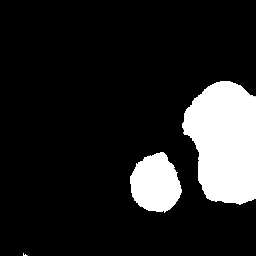
\includegraphics[width=0.18\textwidth]{reports/images/mask.png} & 
        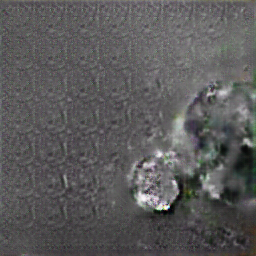
\includegraphics[width=0.18\textwidth]{reports/images/cgan_unet.png} & 
        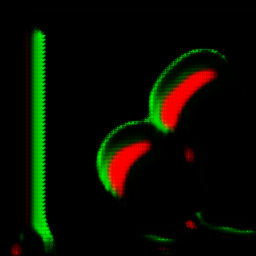
\includegraphics[width=0.18\textwidth]{reports/images/attention_gan_1_cycle.png} & 
        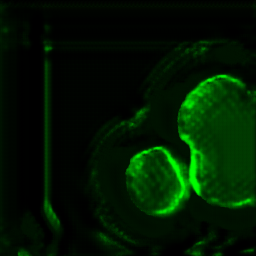
\includegraphics[width=0.18\textwidth]{reports/images/attention_gan_3_cycles.png} & 
        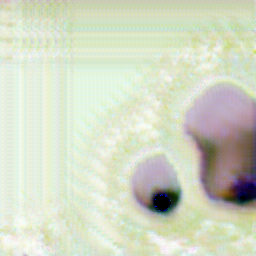
\includegraphics[width=0.18\textwidth]{reports/images/cycle_gan.png} \\
        Synthetic mask & cGAN & AttentionGAN (1 cycle) & AttentionGAN (3 cycle) & CycleGAN
    \end{tabular}
    \caption{Comparative Visualization of Generated Images}
    \label{fig:image_matrix}
\end{figure*}
\subsection{Separate by modalities to balance dataset}
The winner MEDIAR of the NeurIPS competition tried to balance their dataset by over-sampling modalities under-represented. We know that imbalance may cause degradation of the model’s performance for minor modalities. To discover the modalities of the dataset and the associated data, MEDIAR used the encoder embeddings from their phase-1 pretrained model to group the data via the k-means clustering algorithm. They set the number of clusters as 40, which is large enough to sufficiently filter minor modality embeddings. 

\begin{figure}[H]
    \centering
    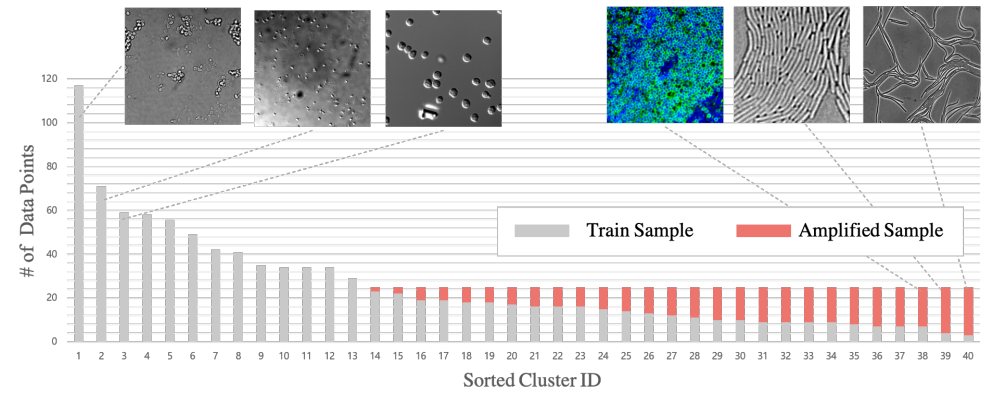
\includegraphics[width=0.6\linewidth]{reports/images/graph_modalities_mediar.png}
    \caption{Discovered modalities and amplified samples in the training dataset by MEDIAR}
\end{figure}

Our work aims to explore new ways to effectively augment data using GANs. In this regard, it seems relevant to follow MEDIAR's approach by dividing our dataset into 40 modalities to achieve a more balanced distribution. However, we intend to apply this strategy to data collected from multiple sources, as previously mentioned, in order to train 40 GANs—one for each modality and its corresponding data. This approach will allow us to augment underrepresented modalities by generating synthetic images that follow the same distribution as their original modality. Such augmentation is expected to result in a more balanced and larger dataset, while preserving data diversity.

\section{Segmentation}
For the actual segmentation task, our most recent progress is training a conditional GAN to generate segmentation masks, conditonnally to the cell image. We achieved a Dice of $0.71$, which ranks around the 30th position on 65 teams on the competition leaderbord on this tuning set.     
Over the next four weeks, once the synthetic data has been generated for the 40 modalities to balance the dataset, we plan to train the baseline U-Net, Cellpose, MEDIAR, YOLO, and SAM-2 models using the original data, the augmented data, the data augmented with GANs, and the data augmented with modality-specific GANs. This will allow us to observe the impact of each type of augmentation.
\end{document}